\documentclass[12pt]{article}
\setlength{\textheight}{24.0cm}
\setlength{\textwidth}{14.5cm}
\setlength{\parindent}{0.0cm}
\setlength{\topmargin}{-1.0cm}
\setlength{\oddsidemargin}{0.0cm}
\renewcommand{\baselinestretch}{1.5}
    
\usepackage{graphicx}
\usepackage{amsmath}
\usepackage{diffcoeff}
\usepackage{amssymb}
\usepackage{subcaption}

% Dash int definitions
\def\Xint#1{\mathchoice
{\XXint\displaystyle\textstyle{#1}}%
{\XXint\textstyle\scriptstyle{#1}}%
{\XXint\scriptstyle\scriptscriptstyle{#1}}%
{\XXint\scriptscriptstyle\scriptscriptstyle{#1}}%
\!\int}
\def\XXint#1#2#3{{\setbox0=\hbox{$#1{#2#3}{\int}$ }
\vcenter{\hbox{$#2#3$ }}\kern-.6\wd0}}
\def\ddashint{\Xint=}
\def\dashint{\Xint-}

\numberwithin{equation}{section}
    
\begin{document}
\thispagestyle{empty}
\Large
\vspace*{2cm}
\begin{center}
    \textbf{UNIVERSITY OF STRATHCLYDE}
\end{center}

\vspace*{1cm}
\begin{center}
    \textbf{DEPARTMENT OF\\ MATHEMATICS AND STATISTICS}
\end{center}

\vspace*{1cm}
\begin{center}
    \textbf{THE N-DIMENSIONAL WAVE EQUATION AND THE METHOD OF DESCENT}
\end{center}

\vspace*{1cm}
\begin{center}
    \textbf{by}
\end{center}

\vspace*{1cm}
\begin{center}
    \textbf{IOANA-TEODORA VADUVA}\\
    \textbf{201444379}
\end{center}

\vspace*{3cm}
\begin{center}
    \textbf{BSc Hons Mathematics}
    \textbf{2017/18}
\end{center}

\newpage
\Large

\vspace*{1cm}
\begin{center}
    \textbf{Statement of work in project}
\end{center}

\vspace*{1cm}
\begin{center}
    \parbox{14cm}{
        The work contained in this project is that of the author and where
        material from other sources has been incorporated full acknowledgement
        is made.}
    \end{center}
    
    \begin{center}
        \begin{tabbing}
            xxxxx\=xxxxxxxxxxxxxxx\= \kill
            \\
            \\
            \\
            \>Signed\>.........................................................\\
            \\
            \>Print Name\>.........................................................\\
            \\
            \>Date\>.........................................................\\
        \end{tabbing}
    \end{center}
    
    \vspace*{5cm}
    Supervised by Dr Marcus Waurick
    \newpage
    \normalsize
    \tableofcontents
    \newpage
    
    \section{Introduction}
    This will be the introduction.
    
    \section{Derivation of the Wave Equation}
    In this section, we will derive the wave equation in one and two dimensions, showing a pattern that 
can be extended to higher dimensions.

\subsection{One Dimension}
The wave equation arises from the movement of string in a musical instrument, such as a guitar or a violin.
\cite{BoyDiP} This string is perfectly elastic and
it is stretched between two supports, at $x=0$ and at $x=L$. The elastic string is of length $L$, as
illustrated in figure \ref{fig:1a}. At time $t=0$, the string is set into motion and left undisturbed to vibrate in the
vertical plane. For this derivation of the wave equation we will simplify things by neglecting damping 
effects such as air resistance.

\begin{figure}[h]
    \begin{subfigure}{0.5\textwidth}
    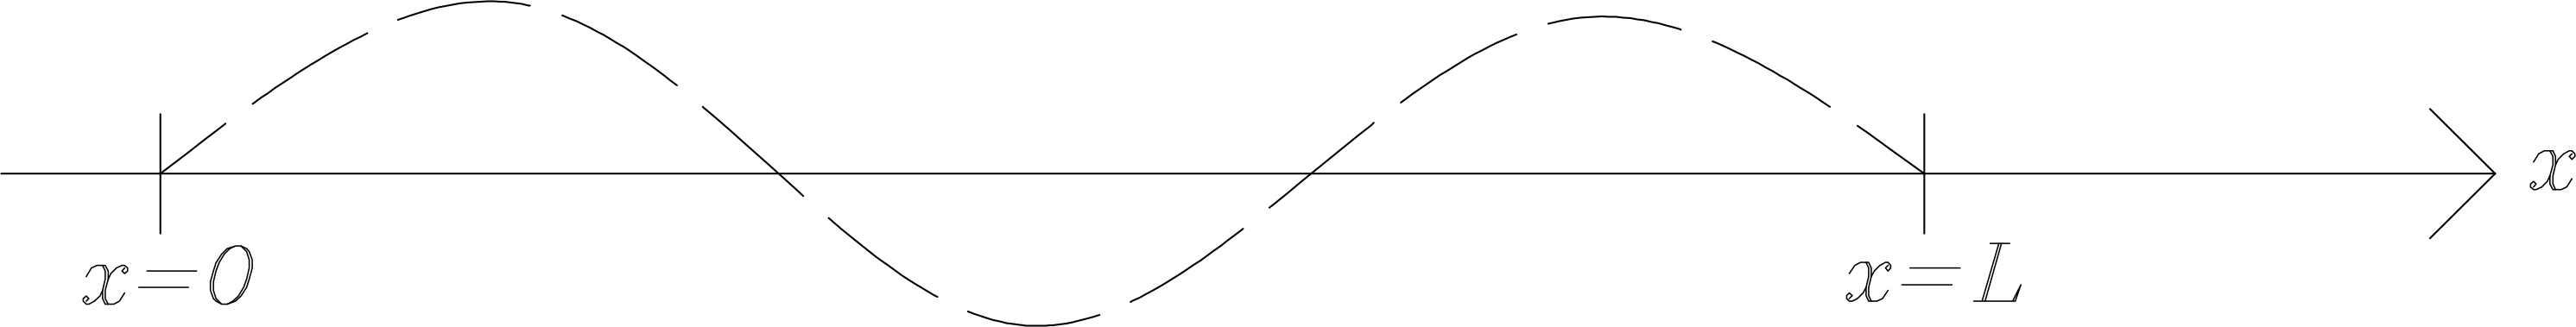
\includegraphics[width=0.9\linewidth, height=5cm]{images/grafic-1} 
    \caption{String of length L}
    \label{fig:1a}
    \end{subfigure}
    \begin{subfigure}{0.5\textwidth}
    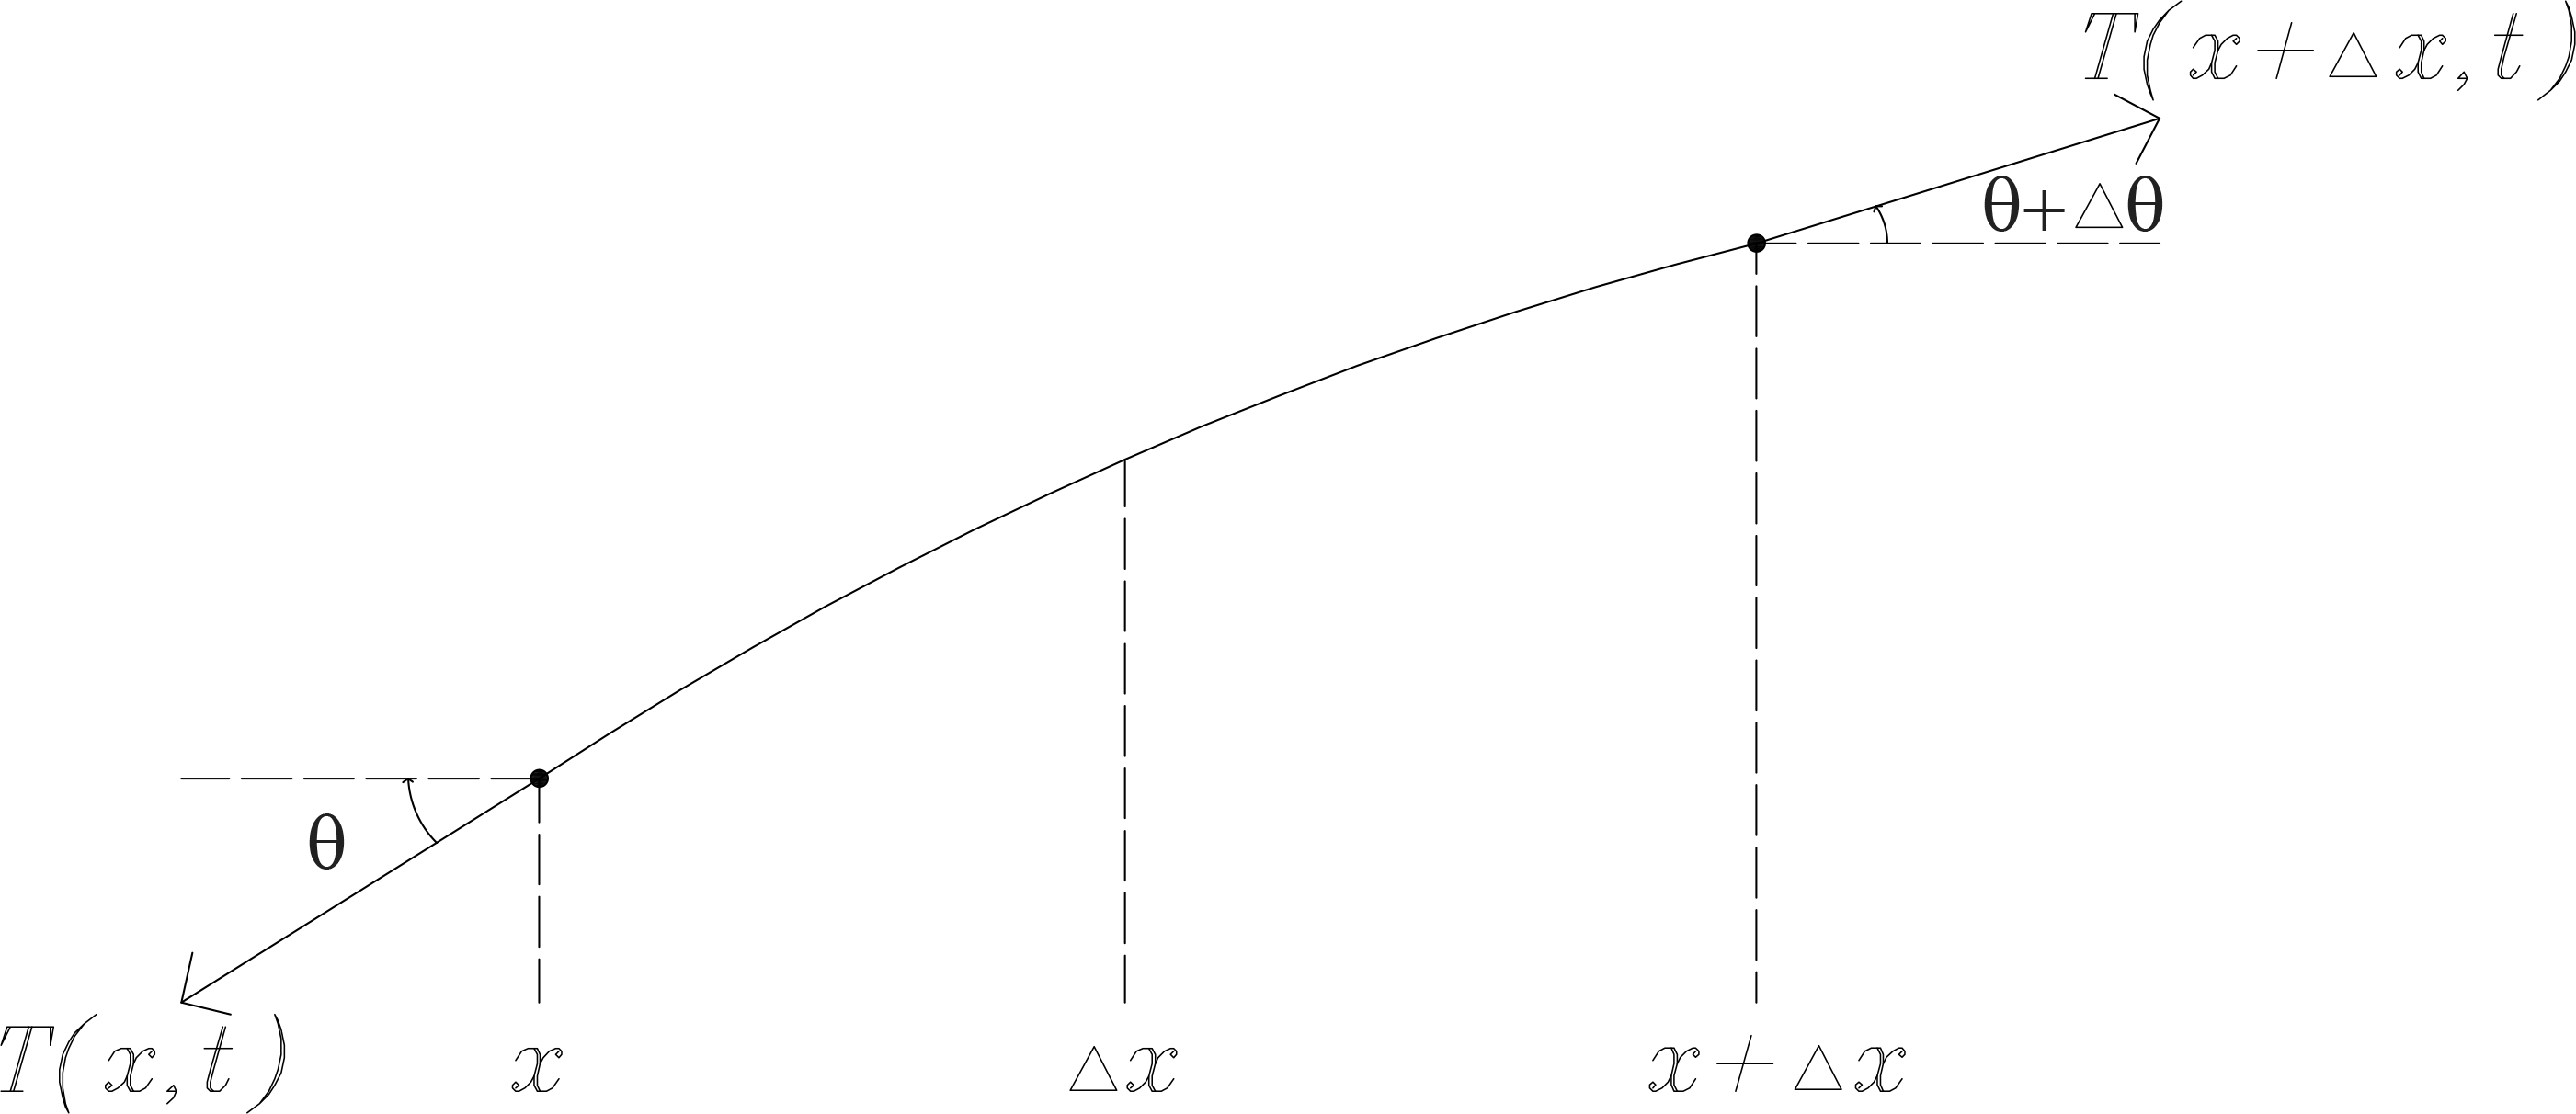
\includegraphics[width=0.9\linewidth, height=5cm]{images/grafic-2}
    \caption{Components of tension}
    \label{fig:1b}
    \end{subfigure}     
\caption{}
\label{fig:1}
\end{figure}

Our aim is to obtain the equation governing this motion. We will obtain this using the Newtonian
mechanics of forces on a small part of the string of length $\Delta x$ which lies between $x$ and 
$x+\Delta x$. The motion of this piece of string is very small and negligible in the horizontal plane
and so we only have movement
in the vertical direction. \cite{Kr} Let $u(x,t)$ be the vertical displacement of point $x$ at the time $t$, 
$T(x,t)$ - the tension in the string that acts only in the direction tangent to the string, and $\rho$ the 
mass per unit length of the string. 
\\

\emph{Newton's Second Law} says that ``for any particle of mass $m$, the net force 
$\boldsymbol{F}$ on the particle is always equal to the mass $m$ times the particle's 
acceleration: $\boldsymbol{F} = m \boldsymbol{a}$.'' \cite{Tay} We apply this to our 
portion of the string $\Delta x$. \emph{Newton's Second Law} applied to our system says that the external
force, the tension at the ends of the string portion, has to equal the product of the mass of the element and 
its acceleration at the mass centre. 
\\

Looking at the movement of the section of string, we see that there is no acceleration in the horizontal direction. 
This is because, as we mentioned before, the movement is insignificant to the system. Therefore, we get the 
following equation governing the horizontal motion:

\begin {equation} \label{eq1}
    T(x+\Delta x,t)\cos{(\theta + \Delta \theta)}-T(x,t)\cos{\theta}=0
\end {equation}

Equation (\ref{eq1}) is obtained by adding together the horizontal components of tension from figure \ref{fig:1b}. Note that the left-hand
side of (\ref{eq1}) is independent of $x$ and we can denote it by $H$ for future reference.
\\

Looking at the vertical movement, we can see that we obtain a similar equation to (\ref{eq1}), with the sole distinction
that now we have a vertical acceleration. This is given by $u_{tt} (\bar{x},t)$, where $u_{tt}$ is the second derivative
of the displacement with respect to time. In physics, the second derivative is equivalent to the acceleration. Here,
 $\bar{x}$ is the coordinate of the centre of mass of the portion of string and $x<\bar{x}<x+\Delta x$. The mass of the 
 section $\Delta x$ is $\rho\Delta x$, and so the vertical movement is given by:

 \begin{equation} \label{eq2}
    T(x+\Delta x,t)\sin{(\theta + \Delta \theta)}-T(x,t)\sin{\theta}=\rho\Delta x u_{tt} (\bar{x},t).
 \end{equation}

 Normally, the weight of the string would also act vertically downwards, but it is neglected here. Similarly to the 
 horizontal case, we can denote the left-hand side of equation (\ref{eq2}) by $V(x,t)=T(x,t)$ and rewrite (\ref{eq2})
 as:

 \begin{equation} \label{eq3}
    \frac{V(x+\Delta x,t)-V(x,t)}{\Delta x}=\rho\Delta x u_{tt} (\bar{x},t)
 \end{equation}

 Taking the limit of (\ref{eq3}) as $\Delta x \rightarrow 0$ (the equivalent of making the string smaller and smaller)
 we get, from the limit definition of the derivative \cite{Spi}, that 

 \begin{equation*}
    \lim_{\Delta x \rightarrow 0}\frac{V(x+\Delta x,t)-V(x,t)}{\Delta x}=V_x(x,t),
 \end{equation*}

i.e. that 
\begin {equation} \label{eq4}
    V_x(x,t)=\rho\Delta x u_{tt} (x,t).
\end{equation}

We want to express equation (\ref{eq4}) in terms of $u$ entirely. Using the definition of the tangent function we see that the vertical movement is the
horizontal movement multiplied by the tangent $V=H\tan{\theta}$. As the derivative with respect to $x$ is the slope of
the tangent \cite{Spi}, we have:

\begin{equation} \label{eq5}
    V(x,t)=H(t)\tan{\theta}=H(t)u_x(x,t).
\end{equation}

Looking back at equation (\ref{eq4}) and combining this with (\ref{eq5}) we obtain that

\begin{equation} \label{eq6}
    V_x(x,t)=(Hu_x)_x.
\end{equation}

Since $H$ is independent of $x$, then (\ref{eq6}) can be written as $V_x(x,t)=Hu_{xx}$, which, by equation (\ref{eq4}), 
gives

\begin {equation} \label{eq7}
    Hu_{xx}=\rho\Delta x u_{tt} (x,t).
\end{equation}

Since the motion of the sting is small, we can replace $H=T\cos{\theta}$ by $T$.\cite{BoyDiP} Hence, (\ref{eq7}) takes the 
form of the one-dimensional wave equation:

\begin{equation} \label{wave}
    c^2u_{xx}=u_{tt}, 
\end{equation}

where $c^2=\frac{T}{\rho}$. We can easily verify that $c$ has the dimensions of 
velocity, as the tension $T$ is a force and $\rho$ is mass divided by length.

\subsection{Two Dimensions} \label{twodim}
In the previous section we looked at how we model a musical instrument string and we obtained the wave equation in 
one dimension, (\ref{wave}). In this section we will see what physical arguments we need to derive the second order wave equation.
In two dimensions, our elastic string is now an elastic, flexible and homogeneous drumhead. Similarly to the string we looked at previously, 
the drumhead has vertical displacement only, i.e. there is no horizontal movement. Furthermore, the area of the membrane we act on is small
compared to the entire drumhead and all angles of inclination are small. \cite{Kr}

\begin{figure}[h]
    \centering
    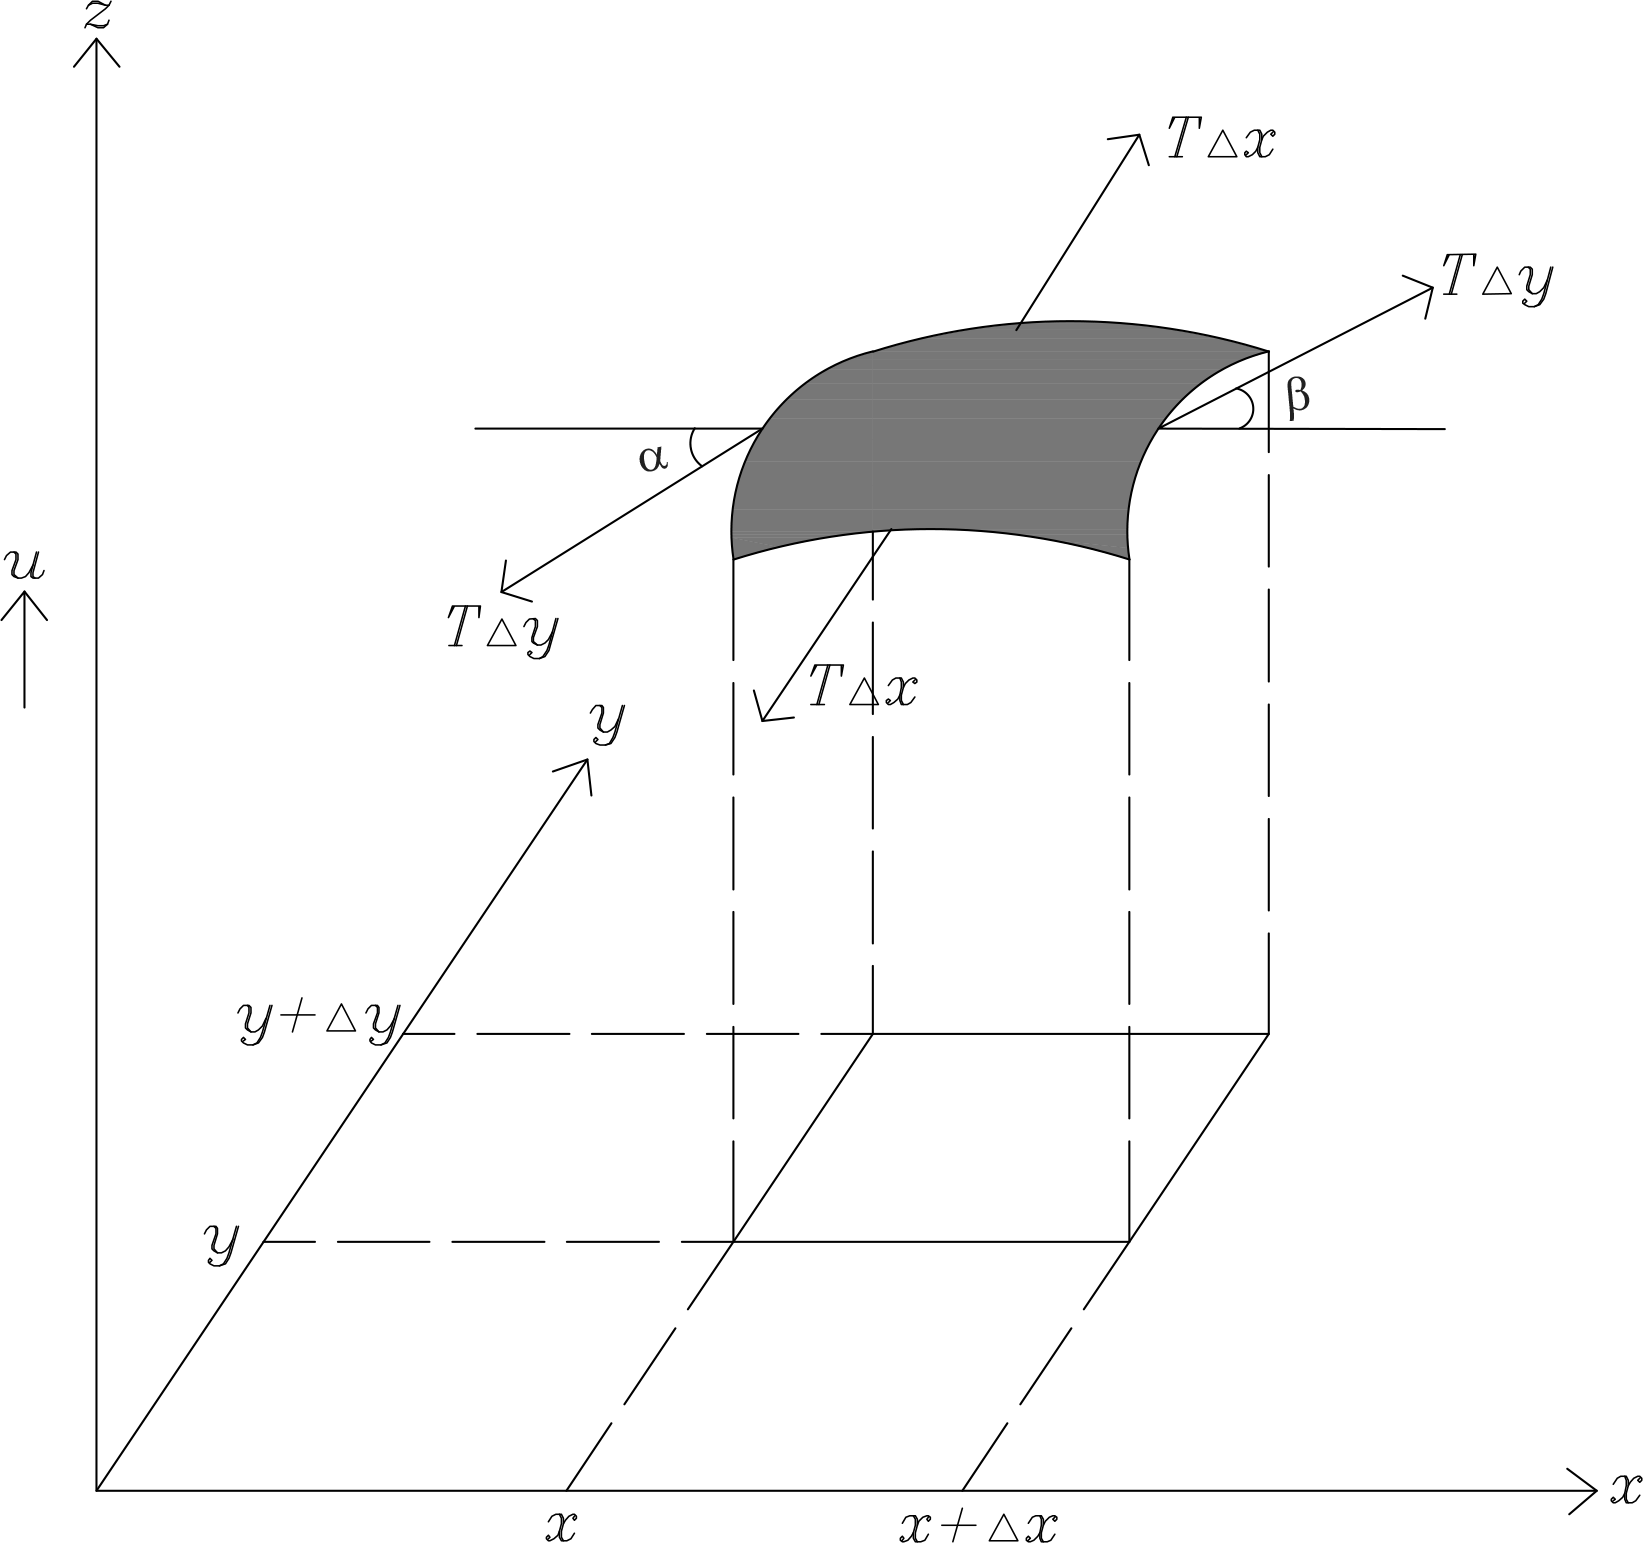
\includegraphics[scale=0.5]{images/grafic-5} 
    \caption{Drumhead membrane}
    \label{fig:2}
\end{figure}

Using \emph{Newton's Second Law}, as before, we obtain that the horizontal components of the tension $T$ are constant and independent of $x$.
Deflections of the membrane and of angles are small, so the sides of the portions are small and approximately equal to $\Delta x$ and $\Delta y$, 
as shown in figure \ref{fig:2}. The tension forces $T$ are acting on the sides of the portion so it is approximately equal to $T\Delta x$ and $T\Delta y$, 
respectively. The forces are tangent to the membrane at all instants as the membrane is perfetly flexible.
\\

We will ignore horizontal movement completly as, like in the one dimensional case, the components are obtained by multiplining the cosines of 
the angles by the forces. However, the angles are very small so we can assume that the cosine values are approximately 1 and the horizontal 
components of the forces at opposite ends of the membrane are approximately equal. This means that the motion is very small and we can ignore it.
\\

The vertical movement is however, more important than the horizontal one. From figure \ref{fig:2} we can see that we have four different components of force.
Firstly, we have the components along the left and right sides given by $T\Delta y \sin\beta$ and $-T\Delta y\sin\alpha$, respectively. As the 
angles are very small, we can replace the sines by tangents \cite{Kr}:

\begin{equation} \label{eq9}
\begin{split} 
    T\Delta y(\sin\beta - \sin\alpha) & \approx T\Delta y(\tan\beta-\tan\alpha)\\
    &= T\Delta y(u_x(x+\Delta x, y_1)-u_x(x, y_2)),
\end{split}
\end{equation}

with $y_1, y_2 \in(y, y+\Delta y)$. Similarly, the vertical components in the other two sides are:

\begin {equation} \label{eq10}
    T\Delta x(u_y(x_1, y+\Delta y)-u_y(x_2,y)),
\end{equation}
where $x_1, x_2 \in(x, x+\Delta x)$.

\emph{Newton's Second Law} with $\rho$ as the mass of undeflected membrane per unit area and $\Delta A=\Delta x\Delta y$ as the area of the portion
of membrane when undeflected, gives the partial differential equation governing this motion:

\begin{equation} \label{eq11}
    T\Delta y\left[u_x(x+\Delta x, y_1)-u_x(x, y_2)]+T\Delta x[(u_y(x_1, y+\Delta y)-u_y(x_2,y)\right]=\rho\Delta x\Delta u_{tt},
\end{equation}

evaluated at some suitable point $(\bar{x},\bar{y})$ corresponding to the section. Divide (\ref{eq11}) by $\rho\Delta x\Delta y$ to obtain:

\begin{equation} \label{eq12}
    \frac{T}{\rho}\left[\frac{u_x(x+\Delta x, y_1)-u_x(x,y_2)}{\Delta x}+\frac{u_y(x_1,y+ \Delta y)-u_y(x_2,y)}{\Delta y}\right]=u_{tt}.
\end{equation}

Letting $\Delta x$ and $\Delta y$ go to zero, both terms in the square bracket of (\ref{eq12}) are the limit definitions of derivatives with
respect to $x$ and $y$ respectively, and so we obtain the formula for the wave equation in two dimensions:

\begin{equation} \label{wave2deq13}
    u_{tt}=c^2(u_{xx}+u_{yy}),
\end{equation}
where, as before, $c^2=\frac{T}{\rho}$. The wave equation in two dimensions (\ref{wave2deq13}) can also be written as $u_{tt}=c^2\Delta^2 u$, 
where $\Delta^2 u=u_{xx}+u_{yy}$ is the \emph{Laplacian} of $u$ in two dimensions.

\subsection{The 3-dimensional Wave Equation}
We can continue with similar arguments to derive the formula for the three dimensional wave equation:

\begin {equation} \label{wave3deq14}
    u_{tt}=c^2(u_{xx}+u_{yy}+u_{zz}).
\end{equation}

This three dimensional equation governs a number of physical processes and phenomenae. Some examples include the vibration of an elastic solid, 
sound waves in air, seismic waves propagating through the Earth, linearised supersonic airflow and electromagnetic waves such as light and radar.
\cite{Str}

\section{Solution in One Dimension}
In this section we will prove the D'Alambert solution to the one dimensional wave equation (\ref{wave}) 
in absence of boundary conditions. The problem we wish to solve is as follows:

\begin{equation} \label{ivp1d}
    \begin{aligned}
    &u_{tt}-c^2u_{xx}=0\\
    &u(x,0)=g(x)\\
    &u_t(x,0)=h(x)
    \end{aligned}
\end{equation}

\subsection{General Form of Solution}

We first begin by showing that the solution has the form $u=\phi(\xi)+\psi(\eta)$, where $\xi=x+ct$ and $\eta=x-ct$. This is quite straightforward
as the operator factorises nicely:

\begin{equation} \label{fact1d}
    u_{tt}-c^2u_{xx}=(\diffp[1]{}{t} - c \diffp[1]{}{x})(\diffp[1]{}{t} + c \diffp[1]{}{x})=0.
\end{equation}

If we denote the last bracket by $v$, we obtain that $v=u_t+cu_x$. Replacing this $v$ into (\ref{fact1d}), we obtain:

\begin{equation*} 
    (\diffp[1]{}{t} -c \diffp[1]{}{x})v=0, \quad \textrm{i.e.} \quad v_t-cv_x=0
\end{equation*}

We now have two first order advection (or in some textbooks, transport) equations:

\begin{equation} 
    \label{veq}
    v_t-cv_x=0 
\end{equation}

\begin{equation}
    \label{ueq}
    u_t+cu_x=v 
\end{equation}

We will first focus on solving (\ref{veq}) using the method of characteristics, a mathematical technique that allows us to transform a partial differential
equation into a simple system of ordinary differential equation. \cite{Ev} The equation (\ref{veq}) is a homogeneous (the right-hand side equals $0$) 
advection equation. Consider $v(x(t),t)$ to be the value of $v$ at time $t$ and position $x(t)$. Then we can use the chain rule to differentiate
$v$ with respect to time:

\begin{equation} \label{diffv}
    \diff{}{t}v(x(t),t)=\diffp[1]{v}{t}+\diffp[1]{v}{x}\diff{x}{t}.
\end{equation}

If we compare (\ref{veq}) and (\ref{diffv}) we obtain that $\diff{v}{t}=0$ if $\diff{x}{t}=-c$. This is our system of two simple ordinary differential 
equations. Solving them each at a time we see that the first one is equivalent to saying that $v$ is constant along the curve $x=x(t)$ for any curve that 
solves the second ODE. We can integrate this and obtain that $x(t)=-ct+x_0$ where $x_0=x$ at time $t=0$ and is just a constant. The equation $x(t)=-ct+x_0$
is the characteristic curve of this differential equation. If we consider the initial condition at $t=0$ in (\ref{ivp1d}) to be $v(x,0)=V(x)$, then the 
solution of (\ref{veq}) is $v(x,t)=V(x+ct)$. We can verify this is true by differentiating $v$ with respect to $t$ and $x$:

\begin{equation*}
    \begin{aligned}
    \diffp[1]{v}{t}=cV'(x+ct)\\
    \diffp[1]{v}{x}=V'(x+ct),
    \end{aligned}
\end{equation*}

which put together give us precisesly (\ref{veq}), and so $v(x,t)=V(x+ct)$ solves (\ref{veq}).
\\

Next, we want to solve (\ref{ueq}), where $v(x,t)=V(x+ct)$. This is now a nonhomogeneous advection equation. Let $w=\diffp[1]{u}{t}-c\diffp{u}{x}$. Then, 
$\diffp[1]{w}{t}+c\diffp{w}{x}=\diffp[2]{u}{t}-c^2\diffp[2]{u}{x}$. This is is precisesly the wave equation from (\ref{ivp1d}). Once again, we have two first
order partial differential equations:

\begin{equation} 
    \label{weq}
    w_t+cw_x=0, 
\end{equation}

\begin{equation}
    \label{ueqw}
    u_t-cu_x=w. 
\end{equation}

We solve (\ref{weq}) in a similar manner to (\ref{veq}), by differentiating $w(x(t),t)$ with respect to time, using the chain rule:

\begin{equation} \label{diffw}
    \diff{}{t}w(x(t),t)=\diffp[1]{w}{t}+\diffp[1]{w}{x}\diff{x}{t}, 
\end{equation}

and comparing with (\ref{weq}). We see once again that $\diff{w}{t}=0$ if $\diff{x}{t}=c$. By the same means from before, we get that the characteristic 
curve of this differential equation is $x(t)=ct+x_0$, where, as before, $x_0$ is $x$ at time $t=0$, and is just a constant. Hence, the solution of (\ref{weq})
is $w(x,t)=W(x-ct)$. As before, we can verify that this solves the equation by differentiating.

We are now close to the result we set off to prove. Consider $\frac{v+w}{2}$:

\begin{equation*}
    \begin{aligned}
    &\frac{v+w}{2}=\frac{1}{2}\left[\diffp[1]{u}{t}-c\diffp[1]{u}{x}+\diffp[1]{u}{t}+c\diffp[1]{u}{x}\right]=\diffp[1]{u}{t},\\
    &\textrm{i.e.} \quad \diffp[1]{u}{t}=\frac{1}{2}\left[V(x+ct)+W(x-ct)\right].
    \end{aligned}
\end{equation*}

When integrating with respect to time, we obtain

\begin{equation} \label{int}
    u(x,t)=\frac{1}{2}\left[\int{V(x+ct)dt}+\int{W(x-ct)dt}\right].
\end{equation}

The first integral in (\ref{int}) is $\phi(x+ct)$ and the second one is $\psi(x-ct)$, such that $\phi'=-\frac{1}{2c}V$ and $\psi'=\frac{1}{2c}W$, respectively.
Therefore, the general solution to the one dimensional wave equation (\ref{ivp1d}) has the claimed form, 
\begin{equation} \label{gensol}
    u=\phi(\xi)+\psi(\eta), \quad \textrm{where} \quad \xi=x+ct \quad \textrm{and} \quad \eta=x-ct.
\end{equation}

\subsection{Solution of the Initial Value Problem}
We now have the general form (\ref{gensol}) of the one dimensional wave equation from (\ref{ivp1d}). In this section, we will use it to derive the solution to
the full initial value problem from (\ref{ivp1d}), where the initial values are $u(x,0)=g(x)$ and $u_t(x,0)=h(x)$. First, set $t=0$ in (\ref{gensol}). This gives:

\begin{equation} \label{t=0}
    u(x,0)=\phi(x)+\psi(x)=g(x).
\end{equation}

Next, we differentiate (\ref{gensol}) using the chain rule, with respect to $t$ to get $u_t(x,t)=c\phi'(x+ct)-c\psi'(x-ct)$. Settin $t=0$ we obtain:

\begin{equation} \label{ut=0}
    u_t(x,0)=c\phi'(x)-c\psi'(x)=h(x).
\end{equation}

For the following calculations we simplify our calculations by changing the variable to something neutral, $s$. 
\\

Differentiate (\ref{t=0}) to get

\begin{equation} \label{eqq9}
    g'(s)=\phi'(s)+\psi'(s).
\end{equation}

Furthermore, divide (\ref{ut=0}) by $c$ to obtain

\begin{equation} \label{eqq10}
    \frac{1}{c}h(s)=\phi'(s)-\psi'(s)
\end{equation}

We will continue by adding and subtracting (\ref{eqq9}) and (\ref{eqq10}). Adding, we obtain

\begin{equation} \label{eqq11}
    \phi'(s)=\frac{1}{2}(g'+\frac{1}{c}h),
\end{equation}

and subtracting gives

\begin{equation} \label{eqq12}
    \psi'(s)=\frac{1}{2}(g'-\frac{1}{c}h).
\end{equation}

Integrating both (\ref{eqq11}) and (\ref{eqq12}) gives:

\begin{equation}
    \begin{aligned}
    \phi(s)=\frac{1}{2}g+\frac{1}{2c}\int^s_0h+A\\
    \psi(s)=\frac{1}{2}g-\frac{1}{2c}\int^s_0h+B.
    \end{aligned}
\end{equation}

Equation (\ref{ut=0}) tells us that by adding (\ref{eqq11}) and (\ref{eqq12}) we have $A+B=0$ which means that $\phi$ and $\psi$ have the
same form. \cite{Str} Substituting $s=x+ct$ for $\phi$ and $s=x-ct$ for $\psi$ we obtain that

\begin{equation}
    u(x,t)=\frac{1}{2}g(x+ct)+\frac{1}{2c}\int^{x+ct}_0h+\frac{1}{2}g(x-ct)-\frac{1}{2c}\int^{x-ct}_0h.
\end{equation}

Rearranging gives the D'Alambert formula to the one dimensional initial value wave equation, developed by the mathematician in 1746: \cite{Str}

\begin{equation} \label{DAla}
    u(x,t)=\frac{1}{2}\left[g(x+ct)+g(x-ct)\right]+\frac{1}{2c}\int^{x+ct}_{x-ct}h(s)ds.
\end{equation}

\subsection{An Application} \label{anapplication}
In this section, we want to present an application to the one dimensional initial value wave equation. We introduce the boundary condition that
$u(0,t)=0$ to the problem in (\ref{ivp1d}) and obtain the boundary value problem:

\begin{equation} \label{bvp1d}
    \begin{aligned}
    &u_{tt}-c^2u_{xx}=0 \quad \textrm {on} \quad \mathbb{R} \times (0,\infty)\\
    &u(x,0)=g(x)\\
    &u_t(x,0)=h(x)\\
    &u(0,t)=0.
    \end{aligned}
\end{equation}

We know how to solve (\ref{ivp1d}), so we will transform (\ref{bvp1d}) into it by extending $u,g,h$ to all of $\mathbb{R}$ by odd reflection. \cite{Ev}
Hence, we define:

\begin{equation*}
    \begin{aligned}
        &\tilde{u}(x,t):=
        \begin{cases}
            u(x,t) \quad \textrm{when} \quad x \ge 0, t \ge 0\\
            -u(-x,t) \quad \textrm{when} \quad x \le 0, t \ge 0\\
        \end{cases}
        \\
        &\tilde{g}(x):=
        \begin{cases}
            g(x) \quad \textrm{when} \quad x \ge 0\\
            -g(-x) \quad \textrm{when} \quad x \le 0\\
        \end{cases}
        \\
        &\tilde{h}(x):=
        \begin{cases}
            h(x) \quad \textrm{when} \quad x \ge 0\\
            -h(-x) \quad \textrm{when} \quad x \le 0,\\
        \end{cases}
    \end{aligned}
\end{equation*}

and so (\ref{bvp1d}) becomes 

\begin{equation*}
    \begin{aligned}
        &\tilde{u}_{tt}=c^2\tilde{u}_{xx} \quad \textrm{in} \quad \mathbb{R}\times(0,\infty)\\
        &\tilde{u}(x,0)=\tilde{g}(x)\\
        &\tilde{u}_t(x,0)=\tilde{h}(x).\\
    \end{aligned}
\end{equation*}

This looks exactly like (\ref{ivp1d}), so we can use the D'Alambert formula (\ref{DAla}) to find a solution for $\tilde{u}$:

\begin{equation*}
    \tilde{u}(x,t)=\frac{1}{2}\left[\tilde{g}(x+ct)+\tilde{g}(x-ct)\right]+\frac{1}{2c}\int^{x+ct}_{x-ct}\tilde{h}(s)ds.
\end{equation*}

Recalling the definitions of $\tilde{u}, \tilde{g}$ and $\tilde{h}$ gives us the solution to (\ref{bvp1d}):

\begin{equation} \label{bvpsol}
    u(x,t)=
    \begin{cases}
        \frac{1}{2}\left[g(x+ct)+g(x-ct)\right]+\frac{1}{2c}\int^{x+ct}_{x-ct}h(s)ds \quad \textrm{if} \quad x \ge t \ge 0\\
        \frac{1}{2}\left[g(x+ct)-g(ct-x)\right]+\frac{1}{2c}\int^{x+ct}_{-x+ct}h(s)ds \quad \textrm{if} \quad 0 \le x \le t\\
    \end{cases}
\end{equation}

We will use the solution (\ref{bvpsol}) to the boundary value wave equation (\ref{bvp1d}) to solve the three dimensional wave equation in 
the next section. Note that if $h \equiv 0$, then (\ref{bvpsol}) can be understood as a plit in the initial displacement, one moving
to the right, and one to the left. \cite{Ev} Furthermore, this solution does not belong to $C^2$, the set of twice differentiable functions, 
unless $g''(0)=0$.

\section{Solution in Three Dimensions}
In this section we will prove the solution to the three dimensional wave equation (\ref{wave3deq14}). In order to do this we will use \emph{spherical
means}, which allow us to transform the partial differential equation into an integral over a sphere of radius $r$, centered at some point $x$. 
Some advantages to using an integral form are that we obtain the solution on the whole domain and that we automatically take into account any
boundary conditions. \cite{Sab} 
\\

The problem we wish to solve is

\begin{equation} \label{3deq}
\begin{aligned}
    &u_{tt}-c^2(u_{xx}+u_{yy}+u_{zz})=0 \quad \textrm{in} \quad \mathbb{R}^3 \times (0,\infty)\\
    &u(x,0)=g(x)\\
    &u_t(x,0)=h(x).\\
\end{aligned}
\end{equation}

We intend, in this section, to derive the formula for $u$ in terms of $g$ and $h$. Our plan is to look at the average of $u$ as 
functions of the time and radius over certain spheres, and apply the D'Alambert formula \ref{bvpsol} from \ref{anapplication}.

\subsection{Some Prerequisite Results} \label{prereq}
As we proceed with our proof of the three dimensional wave equation, we require another important results, which we will not prove, but more information
can be found in Evans' "Partial Differential Equations", \cite{Ev}.
\\

Firstly, we introduce some notation to simplify our future work. Let $x\in \mathbb{R}^n, t>0, r>0$. Then, we have

\begin{equation} \label{averageU}
    U(x;r,t)=\dashint_{\partial B(x,r)}u(y,t)dS(y),
\end{equation}

the average of $u(\cdot,t)$ over the sphere $\partial B(x,r)$. \cite{Ev} Similarly, we have the averages of $g$ and $h$ over the same sphere:

\begin{equation} \label{averageGH}
    \begin{aligned}
        &G(x,r)=\dashint_{\partial B(x,r)}g(y)dS(y)\\
        &H(x,r)=\dashint_{\partial B(x,r)}h(y)dS(y).
    \end{aligned}
\end{equation}

When we fix $x$, we can regard $U$ as a function of just $r$ and $t$. This $U$ solves the \emph{Euler-Poisson-Darbuox equation}. If $u$ satisfies
(\ref{3deq}), then we have $U \in C^m(\bar{\mathbb{R}}_+\times[0,\infty])$, where $\bar{\mathbb{R}}_+$ is the closure of the positive real numbers (i.e.
all the points in $\mathbb{R}_+$ together with all the limit points of this set). The \emph{Euler-Poisson-Darbuox equation} is

\begin{equation} \label{EPDeq}
    \begin{aligned}
        &U_{tt}-c^2U_{rr}-\frac{n-1}{r}U_r=0 \quad \textrm{in} \quad \mathbb{R}_+ \times (0,\infty)\\
        &U=G, \quad U_t=H \quad \textrm{on} \quad \mathbb{R}_+ \times \{ t=0 \}.
    \end{aligned}
\end{equation}
\\

Another piece of mathematics we require for our derivation of solution of the three dimensional wave equation is the transformation formula for surface integrals. That is,
we want to show $\int_{\partial B(x,t)}f(y)dS=t^2\int_{\partial B(0,1)} f(x+tz)dS(z)$. The change of variables formula in $\mathbb{R}^3$ \cite{LooSter} is:

\begin{equation*}
    \int_{\partial B(x,r)}f(y)dS(y)=\int_U f(y(s,t))\left\| \diffp[1]{y}{s} \times \diffp[1]{y}{t} \right \|ds dt
\end{equation*}

The function $f(y)$ can be written as $f(y)=f(x+r(\frac{y-x}{r}))$ such that $y(s,t)$ can be thought of as a parametrisation of any ball $\partial B(x,r)$ for $(s,t)\in U$. Then we can see
that $\frac{y(s,t)-x}{r}$ is a parametrisation of the sphere of radius 1, centred at the origin, $\partial B(0,1)$ for the same $(s,t)\in U$. Furthermore, using these parametrisations, we obtain

\begin{equation*}
    \left \| \diffp[1]{y}{s} \times \diffp[1]{y}{t} \right \| =r^2 \left \| \diffp[1]{}{s}(\frac{y-x}{r}) \times \diffp[1]{}{y-x}{r} \right \|.
\end{equation*}

Letting $z(s,t)=\frac{y(s,t)-x}{r}$, we obtain our required result:

\begin{equation*}
    \begin{aligned}
    \int_U f(y(s,t)) \left \| \diffp[1]{y}{s} \times \diffp{y}{t} \right \| dsdt&=r^2\int_U f(x+rz(s,t)) \left \| \diffp[1]{z}{s} \times \diffp[1]{z}{t} \right \| dsdt\\
    &=r^2\int_{\partial B(0,1)}f(x+rz)dS(z).
    \end{aligned}
\end{equation*}

In our case, $r=t$. This is just a different notation and does not change our result.

\subsection{Kirchhoff's Formula}
We now want to derive the formula for the solution to the wave equation in three dimensions (\ref{3deq}). We will assume that $u \in C^2(\mathbb{R}^3 \times
[0, \infty))$ solves (\ref{3deq}). Denote 

\begin{equation} \label{Udash}
    \tilde{U}:=rU
\end{equation}

\begin{equation} \label{GHdash}
    \begin{aligned}
        &\tilde{G}:=rG\\
        &\tilde{H}:=rH,    
    \end{aligned}
\end{equation}

where $U,G$ and $H$ are defined as in (\ref{averageU}) and (\ref{averageGH}), respectively. Using this notation and the \emph{Euler-Poisson-Darboux equation} we can
obtain the boundary value problem solved in \ref{anapplication}:

\begin{equation*}
    \begin{aligned}
        \tilde{U}_{tt}&=rU_{tt}\\
        &=r\left[c^2U_{rr}+\frac{2}{r}U_r\right] \quad \textrm{by (\ref{EPDeq}) with} \quad n=3\\
        &=c^2rU_{rr}+2U_r\\
        &=(U+c^2rU_r)_r\\
        &=(c^2\tilde{U}_r)\\
        &=c^2\tilde{U}_{rr}.        
    \end{aligned}
\end{equation*}

This means that $\tilde{U}$ solves:

\begin{equation} \label{tilUwave}
    \begin{aligned}
        &\tilde{U}_{tt}-c^2\tilde{U}_{rr}=0 \quad \textrm{on} \quad \mathbb{R}\times (0,\infty)\\
        &\tilde{U}=\tilde{G}, \quad \tilde{U}_t=\tilde{H} \quad \textrm{in} \quad \mathbb{R}\times\{t=0\}\\
        &\tilde{U}=0 \quad \textrm{on} \quad \{r=0\}\times (0, \infty).
    \end{aligned}
\end{equation}

Note that $\tilde{G}_{rr}(0)=0$ as $\tilde{U}(x,0)=\tilde{G}$ in (\ref{tilUwave}). As this boundary value problem is the same as (\ref{bvp1d}), then we can apply 
the solution (\ref{bvpsol}) to (\ref{tilUwave}). Hence, for $0 \le r \le t$ we have 

\begin{equation} \label{newUtil}
    \tilde{U}(x;r,t)=\frac{1}{2c}\left[\tilde{G}(r+ct)-\tilde{G}(r-ct)\right]+\frac{1}{2c}\int^{r+ct}_{-r+ct}\tilde{H}(y)dy.
\end{equation}

Note that our definition of $U$ (\ref{averageU}) implies that $u(x,t)=\lim_{r\rightarrow 0^+}U(x;r,t)$, so our definitions of $\tilde{G}, \tilde{H}$ (\ref{GHdash}),
 and the new expression for $\tilde{U}$ (\ref{newUtil}) lead to

\begin{equation} \label{almostK}
    \begin{aligned}
        u(x,t)&=\lim_{r\rightarrow 0^+}\frac{\tilde{U}(x;r,t)}{r}\\
        &=\lim_{r\rightarrow 0^+}\left[\frac{\tilde{G}(r+ct)-\tilde{G}(r-ct)}{2rc}+\frac{1}{2rc}\int^{r+ct}_{-r+ct}\tilde{H}(y)dy\right]\\
        &=\tilde{G}'(t)+\tilde{H}(t)\\
        &=\diffp[1]{}{t}\left[t\dashint_{\partial B(x,t)}{gdS} \right]+t\dashint_{\partial B(x,t)}{hdS} \quad \textrm{by (\ref{averageGH})}
    \end{aligned}
\end{equation}

Note that in \ref{prereq} we saw that $\int_{\partial B(x,t)}f(\boldsymbol{y})dS=t^2\int_{\partial B(0,1)} f(x+tz)dS(z)$. We will use this to complete our solution of the
three dimensional wave equation:

\begin{equation*}
    \begin{aligned}
    \diffp[1]{}{t}\dashint_{\partial B(x,t)} {g(y)dS} &= \dashint_{\partial B(0,1)} {Dg(x+tz)zdS(z)}\\
    &=\dashint_{\partial B(x,t)}{Dg(y)(\frac{y-x}{t})dS(y)},
    \end{aligned}
\end{equation*}

where $D$ represents the derivative with respect to time. Substituting this into (\ref{almostK}), we obtain the solution to the three dimensional wave equation, which is known as \emph{Kirchhoff's formula}, but is 
actually due to Poisson \cite{Str}:

\begin{equation*}
    u(x,t)=\dashint_{\partial B(x,t)}{th(y)+Dg(y)(\frac{y-x}{t})+g(y)dS(y)}.
\end{equation*}

\section{Solution in Two Dimensions}
In this section we will present the solution to the 2-dimensional wave equation derived in \ref{twodim}. Before we prove the solution, we will discuss \emph{Huygens' 
Principle} and explain why we solved the three dimensional equation first.

\subsection{Huygens' Principle}
\emph{Huygens' Principle} describes how we can physically hear sharp sounds and see sharp images. \emph{Folland} \cite{Fol} gives a very simple example to illustrate 
this. He says that if we are in a dark room at a position $x_0$ that doesn't change, and we set off a flash light at the origin of the three dimensional system we 
created from the room, at time $t=0$, then we will be able to see the light only for as long as it takes it to travel from its position to where we are, the room
becoming dark again after. Another simple example to illustrate \emph{Huygens' Principle} is given by \emph{Strauss} \cite{Str}, where he looks at how the sound
from a musical instrument is heard by the human ear. He says that sound is carried through air at precisesly the fixed speed $c$ without any disturbance by assuming
there are no walls or other inhomogeneities in the air, so that at any time $t$, the listener hears exactly what notes the musical instrument plays at the time $t-\frac{d}{c}$,
where $d$ is the distance between the listener and the instrument, rather than hearing a mixture of notes from earlier echoing over the new notes. These three-dimensional 
examples show phenomenae that are known as \emph{Huygens' Principle}, i.e. it asserts that an initial state is observed at a different place as an effect that is 
very rigorously delimited. \cite{Hil} 
\\

This physical phenomenon makes sense in three dimensions and it is encountered in everyday life. However, we might be interested if a two-dimensional system would follow
the same rules. The answer is no, and an example to show this comes from dropping a pebble into an undisturbed pond. The waves that are created by the pebble satisfy 
approximately well the two-dimensional wave equation with a certain speed $c$, where $x$ and $y$ are horizontal coordinates of the 2D plane. If we assume there exists
a waterbug without any movement, at a distance $d$ from the point of impact between the pebble and the water, it will feel a wave at time $t=d/c$, but that wave will
not stop upon reaching the waterbug, but continue to send out waves. Those secondary waves become so small that they are no longer felt after a period of time, but they 
do not actually ever stop. \cite{Str} This means that \emph{Huygens' Principle} no longer holds. This is because the time does not limit the initial state is not limited 
in time, i.e. once a signal reaches a point in the two-dimensional space, it continues there indefinitely. \cite{Hil}
\\

\emph{Huygens's Principle} allowed us to straightforwardly derive the solution of the three-dimensional equation using spherical means. However, this same principle
means that the same method cannot be employed to solve the two-dimensional equation, but it offers an alternative based on the three-dimensional problem. The trick is
to solve the case in three dimensions and then \emph{descend} into two dimensions by letting the $z$-coordinate equal $0$. \cite{Ev} We shall see how this works in the 
next section. 

\subsection{Poisson's Formula}

\section{Solutions in Higher Dimensions}

\subsection{Odd Dimensions}
\subsection{Even Dimensions}
\subsection{Uniqueness of Solutions}

\section{Conclusion}

\begin{thebibliography}{99}
\bibitem{BoyDiP} Boyce and Di Prima 
\bibitem{Kr} Kreyszig, Advanced Engeneering Methods
\bibitem{Tay} John R. Taylor, Classical Mechanics
\bibitem{Spi} Michael Spivak, Calculus (around pg 150-160)
\bibitem{Str} Strauss, Partial Differential Equations: An Introduction
\bibitem{Ev} Evans, Partial Differential Equations
\bibitem{Sab} Sabelfeld, Spherical Means for PDEs
\bibitem{LooSter} Lynn Loomis, Shlomo Sternberg, Advanced Calculus
\bibitem{Fol} Folland, Introduction to PDEs
\bibitem{Hil} Courant and Hilbert, Methods of Mathematical Physics
\end{thebibliography} (pg3)
\end{document}
